
\documentclass{article}

% Recommended, but optional, packages for figures and better typesetting:
\usepackage{microtype}
\usepackage{graphicx}
\usepackage{subfigure}
\usepackage{booktabs} % for professional tables

\usepackage{amssymb}
\usepackage{amsthm}
\usepackage{amsmath}

\newtheorem{lemma}{Lemma}
\newtheorem{theorem}{Theorem}
\newtheorem{coro}{Corollary}


\theoremstyle{definition}
\newtheorem{definition}{Definition}


\newcommand{\diffusion}{N}
\newcommand{\rotparm}{R}

\newcommand{\latV}{z}
\newcommand{\obsV}{x}

\newcommand{\LEG}{\mathrm{LEG}}
\newcommand{\reals}{\mathbb{R}}
\newcommand{\LEGGP}{\mathrm{LEG}}
\newcommand{\PEG}{\mathrm{PEG}}
\newcommand{\PEGGP}{\mathrm{PEG}}
\newcommand{\KPEG}{\mathrm{KPEG}}
\newcommand{\KLEG}{\mathrm{KLEG}}
\newcommand{\SM}{\mathrm{SM}}
\newcommand{\Cov}{\mathrm{Cov}}
\newcommand{\TODO}{TODO}

% hyperref makes hyperlinks in the resulting PDF.
% If your build breaks (sometimes temporarily if a hyperlink spans a page)
% please comment out the following usepackage line and replace
% \usepackage{icml2019} with \usepackage[nohyperref]{icml2019} above.
\usepackage{hyperref}

% Attempt to make hyperref and algorithmic work together better:
\newcommand{\theHalgorithm}{\arabic{algorithm}}

% Use the following line for the initial blind version submitted for review:
% \usepackage{icml2019}

% If accepted, instead use the following line for the camera-ready submission:
\usepackage[accepted]{icml2019}

% The \icmltitle you define below is probably too long as a header.
% Therefore, a short form for the running title is supplied here:
\icmltitlerunning{Linear-time inference for Gaussian processes on one Dimension}

%comment this line out later, when we're ready to submit - useful to have page numbers visible in draft mode
\pagestyle{headings}

\begin{document}

\twocolumn[
\icmltitle{General linear-time inference for Gaussian Processes on one dimension}

% It is OKAY to include author information, even for blind
% submissions: the style file will automatically remove it for you
% unless you've provided the [accepted] option to the icml2019
% package.

% List of affiliations: The first argument should be a (short)
% identifier you will use later to specify author affiliations
% Academic affiliations should list Department, University, City, Region, Country
% Industry affiliations should list Company, City, Region, Country

% You can specify symbols, otherwise they are numbered in order.
% Ideally, you should not use this facility. Affiliations will be numbered
% in order of appearance and this is the preferred way.

\begin{icmlauthorlist}
\icmlauthor{Jackson Loper}{to}
\icmlauthor{David Blei}{to}
\icmlauthor{John P. Cunningham}{to}
\icmlauthor{Liam Paninski}{to}
\end{icmlauthorlist}

\icmlaffiliation{to}{Columbia University, New York, New York, USA}

\icmlcorrespondingauthor{Jackson Loper}{jl5116@columbia.edu}

% You may provide any keywords that you
% find helpful for describing your paper; these are used to populate
% the "keywords" metadata in the PDF but will not be shown in the document
\icmlkeywords{Gaussian Processes}

\vskip 0.3in
]

% this must go after the closing bracket ] following \twocolumn[ ...

% This command actually creates the footnote in the first column
% listing the affiliations and the copyright notice.
% The command takes one argument, which is text to display at the start of the footnote.
% The \icmlEqualContribution command is standard text for equal contribution.
% Remove it (just {}) if you do not need this facility.

\printAffiliationsAndNotice{}  % leave blank if no need to mention equal contribution
% \printAffiliationsAndNotice{\icmlEqualContribution} % otherwise use the standard text.

\begin{abstract}
Gaussian Processes (GPs) provide a powerful probabilistic framework for interpolation, forecasting, and smoothing, but have been hampered by computational scaling issues.  Here we prove that for data sampled on one dimension (e.g., a time series sampled at arbitrarily-spaced intervals), approximate GP inference at any desired level of accuracy requires computational effort that scales \emph{linearly} with the number of observations; this new theorem enables inference on much larger datasets than was previously feasible. To achieve this improved scaling we propose a new family of stationary covariance kernels: the Latent Exponentially Generated (LEG) family, which admits a convenient stable state-space representation that allows linear-time inference.  We prove that any continuous integrable stationary kernel can be approximated arbitrarily well by some member of the LEG family.  The proof draws connections to Spectral Mixture Kernels, providing new insight about the flexibility of this popular family of kernels.  We propose parallelized algorithms for performing inference and learning in the LEG model, test the algorithm on real and synthetic data, and demonstrate scaling to datasets with billions of samples.
\end{abstract}

\section{Introduction}

Gaussian Process (GP) methods are a powerful and expressive class of nonparametric techniques for interpolation, forecasting, and smoothing.  
However, this expressiveness comes at a cost: if implemented naively, inference in a GP given $m$ observed data points will require $O(m^3)$ operations. 
A large body of work has devised various means to circumvent this cubic run-time; briefly, this literature can be broken down into several threads.  A first approach is to attempt to perform exact inference without imposing any restrictions on the covariance kernel, using careful numerical methods typically including preconditioned conjugate gradients \cite{Cutajar2016}. \citet{Wang2019}
represents the state of the art: inference and learning can be performed on $\sim 10^6$ datapoints on an 8-GPU machine and a few days of processing time.
A second approach searches for good approximations to the posterior that do not rely on special properties of the covariance kernel.  Some well-known examples of this approach include   \cite{quinonero2005unifying,snelson2007local,hensman2013gaussian,low2015parallel,de2017gpflow}.  
In a third approach, several techniques exploit special kernel structure.  Examples include matrices with Kronecker product structure \cite{gilboa2013scaling}, Toeplitz structure \cite{zhang2005time, cunningham2008}, matrices that can be well-approximated with hierarchical factorizations \cite{Ambikasaran2015},
or matrices which are sufficiently smooth to allow for interpolation-based approximations \cite{kiss-gp}.

When the GP has one-dimensional input -- e.g., 
a scalar or vector time-series sampled at arbitrary time points -- the most popular method for scaling learning and inference is to approximate the GP with some form of Gaussian hidden Markov model (that is, a state-space model) \cite{reinsel2003elements,mergner2009applications,cheung2010estimation,brockwell2013time}.  This model class has considerable virtue: it is a particular case of a GP, it includes popular models like the auto-regressive moving average process (ARMA, when on an evenly spaced grid), and perhaps most importantly it admits linear-time $O(m)$ inference via message passing.

Is approximating a GP with a state-space model a generally viable strategy?
In several special cases it has been shown that state-space models provide excellent approximations of specific covariance kernels 
\cite{karvonen2016approximate,benavoli2016state}.  Discrete-time processes on a finite interval can also be approximated this way \cite{lindgren2011explicit}.  Practically, \cite{gilboa2013scaling} shows it is straightforward to learn many GP models using a state-space model. 

In this work we establish the full generality of this strategy: we offer a new theorem proving that \emph{any} GP on one dimension with a Lebesgue-integrable continuous kernel can be arbitrarily well approximated by a specifically-chosen state-space model.  By doing so, we effectively reduce the run-time burden of  GPs on one dimension from cubic to linear.

We first develop a new class of Gaussian hidden Markov models on one dimension: the Latent Exponentially Generated (LEG) process.  This model family is a generalization of the Celerite family of Gaussian Processes \cite{foreman2017celerite}.  Unlike some popular state-space models such as the ARMA, LEG 
processes do not require that the observations are equally spaced.  These models define a distribution on vector-valued functions on the entire real line, $X: \mathbb{R} \rightarrow \mathbb{R}^n$.  By construction, LEG processes are stable and stationary, with a kernel that can be evaluated easily, and
inference requires linear time.  In addition, we here show that inference for these models can be parallelized efficiently via a technique known as Cyclic Reduction \cite{sweet1974generalized}, leading to significant runtime improvements.  Furthermore these models are general: our main mathematical result is to prove that for any stationary Gaussian Process $X$ on one dimension with integrable continuous covariance, for any $\varepsilon$, the covariance of $X$ can be matched within $\varepsilon$ by a 
LEG covariance kernel. 

LEG kernels generalize the Celerite kernel \cite{foreman2017celerite} by allowing more model flexibility and permitting vector-valued observations.  Every Celerite kernel can be understood as a special case of a LEG kernel.   

The remainder of this paper defines the LEG family, derives its essential properties and generality, and finally empirically backs up these claims across real and synthetic data.  In particular, we show that the LEG family enables inference on datasets with billions of samples with runtimes that scale in minutes, not days.  


%                  _   _     
%                 | | | |    
%  _ __ ___   __ _| |_| |__  
% | '_ ` _ \ / _` | __| '_ \ 
% | | | | | | (_| | |_| | | |
% |_| |_| |_|\__,_|\__|_| |_|
                           
\section{Preamble: Gaussian process generalities}

A Gaussian Process on one dimension is a random function $X: \reals \rightarrow \reals^n$ such that for any finite collections of times $t_1,t_2\cdots t_m$ the joint distribution of $(X(t_1),\cdots X(t_m)) \in \mathbb{R}^{m\times n}$ is jointly Gaussian.  The covariance kernel of $X$ is a matrix-valued function defined by 
\[
\Sigma(s,t) = \Cov(X(s),X(t)) \in \reals^{n\times n}.
\]
A process is said to be stationary if $\Sigma(s,t)=C(s-t)$ for some matrix-valued function $C$ and $\mathbb{E}[X(t)]$ is the same for all values of $t$.  In this case we write $\tau$ for the time-lag $t-s$, i.e $C=C(\tau)$.  

We will focus on two critical computational tasks here: inference and learning.  
``Inference" refers to using a GP model to compute the conditional densities of  $X$ given a finite collection of observations $D=(X(t_1),\cdots X(t_m))$.  ``Learning" refers to estimating the covariance of $X$ from the data $D$.  Both of these tasks can be computationally intensive: naive evaluation of the likelihood of $D$ requires computing the determinant of an $m\times m$ matrix and solving an $m$-dimensional linear system.
In general these tasks require $O(m^3)$ operations.  Here we circumvent this scaling law by restricting ourselves to a parametric family of kernels which admit linear-time (i.e., $O(m)$) algorithms.  We further show that this restriction is without loss of generality, since this family of kernels is capable of approximating any integrable continuous stationary kernel on the real line.


\section{The LEG kernel}

We introduce a parametric family of random processes on one dimension: the Latent Exponentially Generated (LEG) process. This process will achieve both goals of this work: linear-time inference and arbitrary approximation quality to any GP. For clarity of exposition, what follows assumes stationarity and zero mean; generalizations are discussed in Section \ref{sec:extensions}.  We first define the latent GP, after which we define the observation model; taken together these objects will form the LEG family.

In designing a family of latent GP models, 
our first goal is to enable fast computation:
the models should be stationary, with an easily-computed kernel.  In addition, it is convenient to focus on Markovian models, since the Markov property will enable efficient inference.

A general and classic family of Markovian models are given by linear Langevin equations \cite{coffey2004langevin}, i.e. processes defined by 
\[
z(t) = z(0) + \int_0^t (-G z(s) ds + \sigma dw(s)),
\]
where $w$ is an $\ell$-dimensional Brownian motion, and $G,\sigma$ are square matrices.  To ensure this process doesn't grow without bound, we need the real part of the eigenvalues of $G$ to be positive.  Guaranteeing this nontrivial constraint is challenging \cite{buesing2012learning,Gillis2019}.  To remedy this problem we developed a closely-related family of models which are always stable and stationary:

\begin{definition} Let $\latV(0) \sim \mathcal{N}(0,I)$, let $w$ denote a Brownian motion, let $\diffusion,\rotparm$ be any $\ell\times \ell$ matrices, and let $G=\diffusion \diffusion^\top + \rotparm-\rotparm^\top$.  Let $\latV$ satisfy
\[
\latV(t) = \latV(0) + \int_0^t\left(-\frac{1}{2}G \latV(s)ds + N dw(s)\right).
\]
Then we will say $z$ is a Purely Exponentially Generated process, $z \sim \PEGGP(\diffusion,\rotparm)$.
\end{definition}

This family has another advantage: the covariance kernel is easy to compute.  The covariance kernel for linear Langevin models usually involves an integral \cite{vatiwutipong2019alternative}, but for PEG models we can compute this 
integral in closed form:
\begin{lemma} $z \sim \PEGGP(\diffusion,\rotparm)$ is stationary, with covariance kernel given by
\[
C_{\PEG}(\tau;\diffusion,\rotparm)  \triangleq
\exp\left(-\frac{\tau}{2}\left(\diffusion \diffusion^\top + \rotparm-\rotparm^\top\right)\right).
\]
\end{lemma}
{\bf Proof:} See supplementary material.  

\begin{figure*}[ht]
\vskip 0.2in
\begin{center}
\centerline{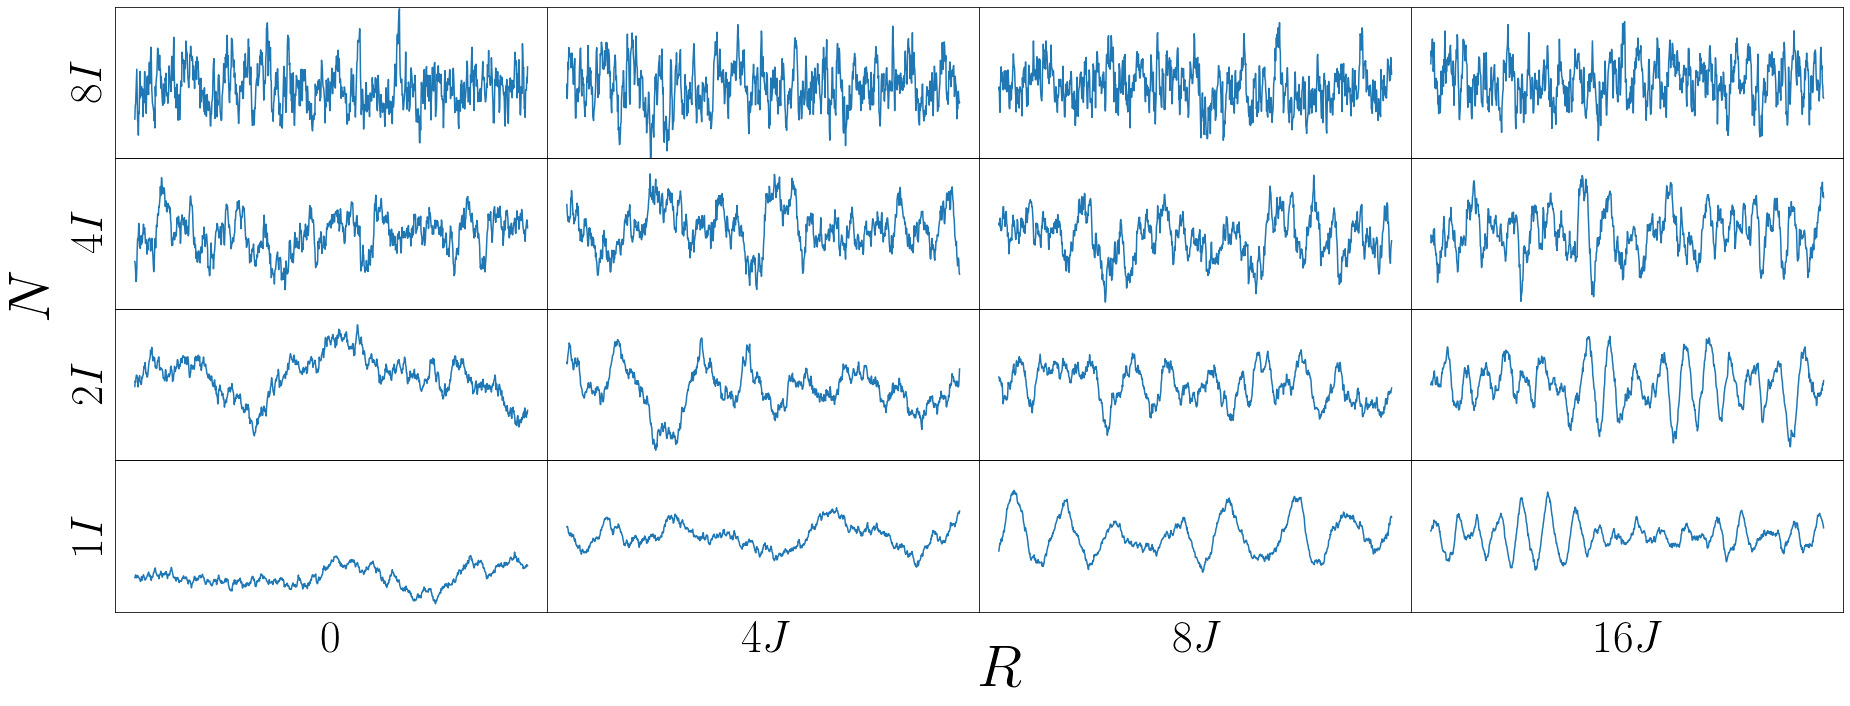
\includegraphics[width=2\columnwidth]{pics/exampleprocs}}
\caption{\textbf{PEG process samples}.  The plots above show representative samples from the model $\PEG(\diffusion,\rotparm)$ as we vary $\diffusion$ and $\rotparm$.  Here we consider rank-2 PEG models (only one element of the 2d vector is plotted), so $\diffusion,\rotparm$ are both $2\times 2$ matrices.   We vary $\diffusion$ by taking it to be various multiples of the identity.  We vary $\rotparm$ by taking various multiples of $J$, the antisymmetric $2\times 2$ matrix with zeros on the diagonal and $\pm 1$ on the off-diagonal.  In this simple rank-2 case, increasing $N$ leads to a less predictable process and  increasing $\rotparm$ leads to faster oscillations.
\label{fig:exampleprocs}}
\end{center}
\vskip -0.2in
\end{figure*}
 

The matrices $\diffusion,\rotparm$ can be interpreted intuitively.  The positive definite diffusion $\diffusion \diffusion^\top$ controls the predictability of the process: when an eigenvalue of $\diffusion \diffusion^\top$ becomes larger, the process $Z$ becomes less predictable along the direction of the corresponding eigenvector.  The antisymmetric  $\rotparm-\rotparm^\top$ term affects the process by applying an infinitesimal deterministic rotation at each point in time.  The eigenvalues of $\rotparm - \rotparm^\top$ are purely imaginary, and when they are large they lead to rapid oscillations in the process, while the eigenvectors control how these oscillations are mixed across the dimensions of $Z$.  As an illustration, Figure \ref{fig:exampleprocs} shows the first dimension of samples from an $\ell=2$ dimensional PEG process with various values of $\diffusion,\rotparm$.

We now turn to the observed process: 

\begin{definition}
Let $\latV \sim \PEGGP(\diffusion,\rotparm)$.  Fix any $n \times \ell$ matrix $B$ and any $\ell \times \ell$ matrix $\Lambda$.   For each $t$ independently, define the conditional observation model: 
\[
\obsV(t)|\latV(t) \sim \mathcal{N}(B \latV(t),\Lambda \Lambda ^\top).
\]
We define a \textbf{Latent Exponentially Generated (LEG)} process to be the Gaussian Process $x: \reals \rightarrow \reals^n$ generated by a PEG prior and the above observation model.  We write $x \sim \LEGGP(\diffusion,\rotparm,B,\Lambda)$.  X has a LEG kernel:
\begin{gather*}
C_\LEG(\tau;\diffusion,\rotparm,B,\Lambda) \\ \triangleq
B \left(C_\PEG(\tau;\diffusion,\rotparm)\right) B^\top + \delta_{\tau=0} \Lambda \Lambda^\top.
\end{gather*}
Here $\delta$ is the indicator function, and again $\tau>0$.  We will refer to the latent dimension $\ell$ as the \textbf{rank} of the LEG kernel.
\end{definition}

\subsection{Computation with LEG processes}

\label{subsec:leggpcomputation}

The LEG model is a Gaussian hidden Markov model.  As usual in such models, it follows that problems of evaluation, interpolation, smoothing, and sampling reduce to operations with block-tridiagonal matrices \cite{de1988likelihood}.  This block-tridiagonal structure is what enables linear-time inference. 

While the obvious choice for processing these block-tridiagonal matrices might be a Kalman filter, it is not ideally suited for modern hardware: the na\"ive Kalman filter requires a single sequential sweep through the data.  If the latent process has a quick mixing time this requirement can be relaxed \cite{gonzalez2009residual}, but we seek an algorithm that parallelizes efficiently regardless of the parameters of the model.  

We here propose to use Cyclic Reduction (CR) techniques instead.  These offer a convenient parallelizable approach to computation with block-tridiagonal matrices \cite{sweet1974generalized}.  To our knowledge, the CR approach has not previously been applied in the Gaussian Process literature. 
Like the Kalman filter, CR can be understood as a linear-time Cholesky decomposition algorithm for block-tridiagonal matrices \cite{eubank2002equivalence}.  Linear-time Cholesky decompositions lead directly to linear-time algorithms for solving linear systems and computing the determinant, which, in turn, allows us to compute all quantities required for inference in LEG processes. The difference between the Kalman filter and CR is ``pivoting''; CR computes the Cholesky decomposition of a carefully permuted version of a block-tridagonal matrix.  This pivoting allows the CR algorithm to proceed in $\log_2 m$ parallelizable stages, each stage concerning a matrix half the size of the matrix from the previous stage\footnote{Those familiar with the multigrid technique \cite{terzopoulos1986image,hackbusch2013multi} -- which has been used for Gaussian inference in other contexts \cite{papandreou2010gaussian,mukadam2016gaussian,zanella2017analysis} -- will note similarities between multigrid and CR.}.   Unlike the Kalman Filter, CR can be completed with $k$ processors on the order of $m/k$ time (as long as $k<m$).   Implementing parallel versions of CR in modern software libraries (TensorFlow2 in this case) was straightforward, making it easy to take advantage of modern hardware.  

Exact linear-time algorithms for likelihood (and gradient) evaluation, smoothing, forecasting, and interpolation are given in the supplement.  TensorFlow2-based Python code, tutorial  notebooks, and API documentation can be found at \url{https://github.com/jacksonloper/leg-gps}. 

\subsection{Generality of the LEG family}
\label{sec:smk}
The LEG family is useful only in so much as it is able to accurately approximate other GP kernels.  Here, we prove that in fact the LEG family is general: \emph{any} stationary Lebesgue-integrable stationary continuous kernel can be approximated to arbitrary accuracy with a LEG family of a certain rank $\ell$.  

Intuitively the argument is as follows: first, the PEG family provides a general and well-behaved (stable, stationary, correlated) collection of $\ell$ state-space components.  Second, the LEG observation model creates 
\emph{mixture} 
of those underlying PEG components.  Third, we show that the LEG family has nonzero intersection with spectral mixture kernels (a popular class of kernels defined more carefully below), thus drawing a novel and useful connection between spectral mixtures and state space models. Fourth, we extend known facts about the generality of spectral mixtures to the multidimensional case.  As a result, finally, we conclude that the LEG family is general (all without sacrificing its linear runtime).

To begin, we study the spectral representation of the LEG kernel.  If a kernel is stationary and continuous, Bochner's theorem guarantees it has a spectrum \cite{bhatia2015positive}: a unique matrix-valued measure $F$ such that
\[
C(\tau) = \int e^{-i\tau \omega } dF(\omega).
\] 
Spectral Mixture (SM) methods offer a direct way to approximate any stationary kernel through its spectrum.    For the purposes of this article we will define SM kernels as follows:  

\begin{definition}
    Let $p$ denote a probability density on $\mathbb{R}$, let $b_1, b_2 \cdots b_{\ell} \in \mathbb{C}^{n}$, let $\mu \in \mathbb{R}^{\ell}$, and let $\gamma>0$.  The \textbf{Spectral Mixture} kernel, $C_\SM(t;p,b,\mu,\gamma)$, is given by 
    \begin{gather*}
     \sum_{k=1}^{\ell}\int e^{-i\xi x}   b_k b_k^* \gamma p(\gamma(\xi - \mu_k)) d \xi.
    \end{gather*}
    We will say that $C$ is \textbf{based on $p$}, since its spectrum is a sum of scaled and shifted versions of $p$.
\end{definition}

Spectral Mixtures were first introduced in machine learning in \cite{wilson2013gaussian}, where it was noted that any kernel which is the covariance of a weakly stationary mean square continuous random process $X:\ \mathbb{R} \rightarrow\mathbb{R}$ (or indeed $X:\ \mathbb{R}^n \rightarrow\mathbb{R}$) can be well-approximated using SM kernels.    
However, that result does not hold for our case, i.e.\ kernels for processes of the form $X:\ \mathbb{R} \rightarrow\mathbb{R}^n$.  In this situation the spectrum of the kernel becomes a complex-matrix-valued measure (instead of an ordinary probability measure).

These mixture kernels have an interesting connection to LEG kernels: all Cauchy-based spectral mixture kernels are actually also LEG kernels.  These kernels thus fall at the intriguing intersection of Gaussian Hidden Markov models (which are linear run-time) and Spectral Mixture models (which have not previously been considered linear run-time).  Every Cauchy-based SM kernel can be understood as a LEG kernel.  There is also another generalization of Cauchy-based SM kernels, known as the Celerite kernels \cite{foreman2017celerite}; these are built by linear combinations of kernels called Celerite terms.  Below we summarize the relationship between these three families of kernels:

\begin{lemma}[SM kernels, Celerite kernels, LEG kernels] \label{lem:smareleg}
\hspace{.01in}

\begin{enumerate}
    \item Every Cauchy-based real-valued SM kernel $C_\SM:\ \mathbb{R} \rightarrow\mathbb{R}$ can be understood as a Celerite kernel.  
    \item Every positive-definite Celerite term can be understood as a LEG kernel.
    \item Every Cauchy-based real-valued SM kernel $C_\SM:\ \mathbb{R} \rightarrow\mathbb{R}^{n \times n}$ can be understood as a LEG kernel.
\end{enumerate}
\end{lemma}

{\bf Proof:} See supplementary material.  

Thus, to prove that the family of LEG kernels is general, it suffices to show that SM kernels are general.  
 The key idea is to generalize a classic result from kernel density estimation.  We achieve this generalization in the following theorem:  

\begin{theorem}[Total variation convergence for weighted kernel density estimation] \label{lem:kdereg}
Let $K,p$ denote bounded densities on $\mathbb{R}^d$.  Let $g:\ \mathbb{R^d} \rightarrow [-M,M]$.  Let $\gamma_\ell = \ell^{1/2d}$.  Let $\mu_1,\mu_2 \cdots \sim p$, independently.  For each $\ell \in 1,2,\cdots$, define  
\[
h_{\ell}(\xi) = \frac{1}{\ell} \sum_{k=1}^{\ell}g(\mu_k) \gamma^d_\ell K(\gamma_\ell(\xi - \mu_k)).
\]
Then
\[
\mathbb{P}\left(\lim_{\ell \rightarrow \infty} \int |h_{\ell}(\xi) - p(\xi)g(\xi)| d\xi  = 0\right) = 1.
\]
\end{theorem}

{\bf Proof:} See supplementary material.  
% All proofs are deferred to the supplement.  

With this theorem in place, we next show that spectral mixture kernels can approximate any integrable continuous kernel for a stationary Gaussian process on one dimension: 

\begin{coro}[Flexibility of Spectral Mixture kernels]
Fix $p$, a bounded probability density on $\mathbb{R}^n$, $\varepsilon>0$, and any Lebesgue-integrable continuous positive definite\footnote{The requirements of continuity and integrability are slightly too strong.   For example, the sinc kernel is not Lebesgue integrable, but it is easy to approximate with a spectral mixture kernel.  In the future we hope to refine these conditions.}  stationary kernel $\Sigma:\ \mathbb{R} \rightarrow \mathbb{C}^{n\times n}$.   There exists a real valued kernel $C=C_\SM(p,b,\mu,\gamma)$ such that $\Vert C(\tau)z -\Sigma(\tau)z \Vert < \varepsilon \Vert z \Vert$ for every $\tau\in\mathbb{R},z\in\mathbb{C}^n$.  
\end{coro}

{\bf Proof:} See supplementary material.  

This corollary can be used to establish our main mathematical result, i.e., that LEG models enjoy the same flexibility guarantee.  

\begin{theorem}[Flexibility of LEG and Celerite kernels] \label{thm:legflex}
For every $\varepsilon>0$ and every Lebesgue-integrable continuous positive definite stationary kernel $\Sigma: \mathbb{R} \rightarrow \mathbb{R}^{n\times n}$ there exists a Celerite kernel  $C$ such that $\Vert C(\tau)z -\Sigma(\tau)z \Vert < \varepsilon \Vert z \Vert$ for every $\tau>0,z\in\mathbb{C}^n$.   Moreover, there exists a LEG kernel with the same guarantee.
\end{theorem}

{\bf Proof:} See supplementary material.  

In conclusion, we have proven that any stationary Gaussian Process on one dimension can be well approximated using LEG processes, and further that the computational effort for LEG processes scales linearly with the number of observations.  Thus, putting these two pieces together, approximate inference for any stationary Gaussian Processes on one dimension, at any desired level of accuracy, requires computational effort that scales linearly with the number of observations.


%           _                 _                 
%   _____  _| |_ ___ _ __  ___(_) ___  _ __  ___ 
%  / _ \ \/ / __/ _ \ '_ \/ __| |/ _ \| '_ \/ __|
% |  __/>  <| ||  __/ | | \__ \ | (_) | | | \__ \
%  \___/_/\_\\__\___|_| |_|___/_|\___/|_| |_|___/
                                               

\section{Extensions}

\label{sec:extensions}

Before moving on to illustrate these results with experiments on simulated and real data, we pause to note several useful extensions.

\subsection{Non-stationary processes}  
We have focused on stationary processes here for simplicity.  A number of potential extensions to non-stationary processes are possible while retaining linear-time scaling.  As one example, 
starting with LEG processes as a base, nonstationary models can be developed using the techniques from \cite{benavoli2016state}.  

\subsection{Non-Gaussian observations}  
Many approaches have been developed to adapt GP inference methods to non-Gaussian observations, including Laplace approximations, expectation propagation, variational inference, and a variety of specialized Monte Carlo methods \cite{hartikainen2011sparse,riihimaki2014laplace,nguyen2014automated,nishihara2014parallel}.  Many of these can be easily adapted to the LEG model, using the fact that the sum of a block-tridiagonal matrix (from the precision matrix of the  LEG prior evaluated at the sampled data points) plus a diagonal matrix (contributed by the likelihood term of each observed data point) is again block-tridiagonal, leading to linear-time updates \cite{smith2003estimating,Paninski2010,fahrmeir2013multivariate,polson2013bayesian,Khan,Nickisch}.


\subsection{Non-linear domains}
Just as Gaussian Markov models in discrete time can be easily extended to Gaussian graphical models on general graphs, we can extend the Gaussian Markov PEG and LEG processes to stochastic processes on more general domains.  In the simplest case the domain of the process could be a tree, with the PEG kernel defined in terms of distance along the tree, rather than distance on the line.  Inference in the resulting tree-structured Gaussian graphical model can proceed via message passing in $O(m)$ time.

\subsection{Multi-dimensional domains}
We can also use LEG kernels to model processes of the form $x:\ \mathbb{R}^d\rightarrow\mathbb{R}^n$.  Let $B,\Lambda$ be matrices, let $N,R$ be collections of matrices, and let $C_\KLEG(\tau;N,R,B,\Lambda) \triangleq \delta_\tau \Lambda \Lambda^\top+ \sum_{r=1}^{\zeta} \prod_{k=1}^d B C_\PEG(\tau_k;N_{rk},R_{rk})B^\top$.   
\begin{theorem}
Let $\Sigma:\ \mathbb{R}^d \rightarrow \mathbb{R}^{n \times n} $ any positive-definite integrable continuous stationary kernel, and fix $\varepsilon>0$.  There exists a KLEG kernel such that $\Vert C(\tau)z-C_\KLEG(\tau)z\Vert < \varepsilon z$. 
\end{theorem}
{\bf Proof:} See supplementary material.  

Efficient computation is possible for observations from a KLEG process along a (potentially irreguarly-spaced) grid.  The covariance matrix of these observations has structure which can be leveraged for efficient computation.  For example, in the supplement we give an algorithm for multiplying by this matrix, and show that the computational cost of this algorithm scales linearly with the number of points in the grid.  Combined with GPyTorch (cf.\ \cite{gardner2018gpytorch}), this algorithm should yield efficient inference algorithms for KLEG processes.



%                            _                      _       
%                           (_)                    | |      
%   _____  ___ __   ___ _ __ _ _ __ ___   ___ _ __ | |_ ___ 
%  / _ \ \/ / '_ \ / _ \ '__| | '_ ` _ \ / _ \ '_ \| __/ __|
% |  __/>  <| |_) |  __/ |  | | | | | | |  __/ | | | |_\__ \
%  \___/_/\_\ .__/ \___|_|  |_|_| |_| |_|\___|_| |_|\__|___/
%           | |                                             
%           |_|                                             


\section{Experiments}

Here we are interested in testing the theoretical results described above.  In practice, how fast is inference with the LEG process?  How well can the LEG model approximate popular kernels?  How well does the LEG model extrapolate and interpolate?  How well can it smooth?

\subsection{Computational complexity}

\begin{figure}[t!]
\vskip 0.2in
\begin{center}
\centerline{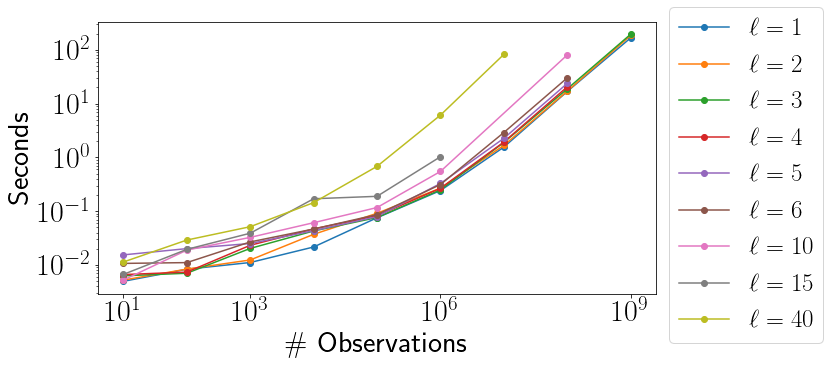
\includegraphics[width=\columnwidth]{pics/scaling}}
\caption{\textbf{Walltime for evaluating LEG likelihoods}.  How long does it take to compute the likelihood of observations from a LEG model on an m5.24xlarge machine on the Amazon AWS service?   We compare times for differently-ranked models and different numbers of observations.   For example, the likelihood for one billion observations under a rank-3 LEG model can be computed in roughly three and a half minutes.  
\label{fig:sofast}}
\end{center}
\vskip -0.2in
\end{figure}


\begin{figure*}[t!]
%\vskip 0.2in
\begin{center}
\centerline{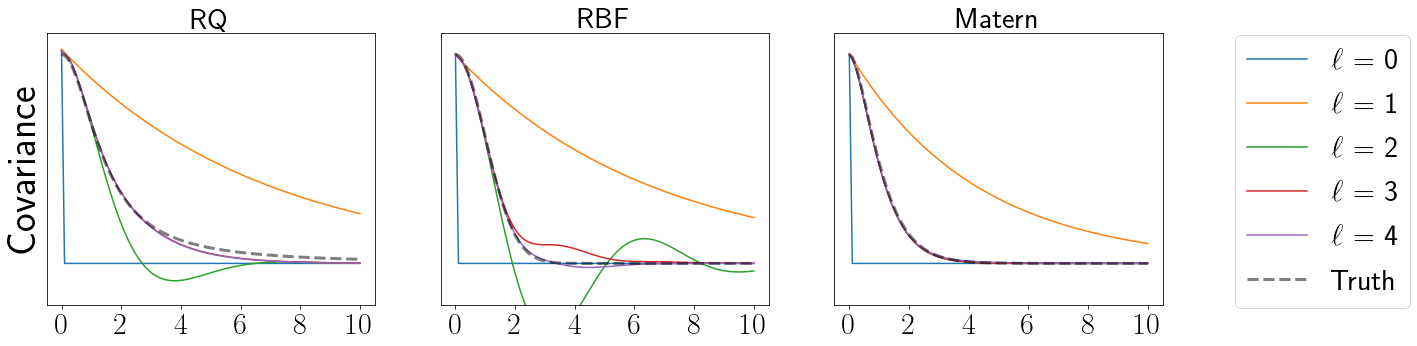
\includegraphics[width=2\columnwidth]{pics/kernelfriends}}
\caption{\textbf{LEG kernel approximation of some popular specific kernels}.  
By taking the rank $\ell$ sufficiently high we can achieve arbitrarily good approximations to any kernel.  In the three examples shown here, $\ell=4$ already provides adequate approximation quality.  Note that in some cases some lines aren't visible because they are superimposed on each other; for example, when approximating Matern kernels we find nearly identical models for for $\ell \in {2,3,4}$.}
\label{fig:reppower}
\end{center}
%\vskip -0.2in
\end{figure*}

Throughout what follows, we will perform inference on LEG processes using the Cyclic Reduction algorithm outlined in \ref{subsec:leggpcomputation}. We wanted to check if there are practical difficulties that could negate the theoretically linear computational cost of this method.  We measured how long it took to compute the likelihood of single contiguous chains of observations from LEG processes of various ranks.  In each case we used an m5-24xlarge machine on Amazon Web Services (AWS).



Overall, the empirical scaling appeared consistent with the theoretical predictions.  The likelihood of one million observations from a rank-3 model could be computed in $0.25$ seconds, and one billion observations could be computed in 195 seconds.  We saw similar trends across models of other ranks; the results are summarized in Figure \ref{fig:sofast}.  Note that for smaller datasets we actually observed a sublinear scaling (i.e. a slope of less than one on the log-log plot) that turns approximately linear for larger values of $m$.


\subsection{Matching one-dimensional kernels}



Theorem \ref{thm:legflex} shows that LEG kernels can represent any stationary Gaussian process arbitrarily well \emph{if} the latent dimension $\ell$ is sufficiently high.  How high does this dimension actually need to be in order to get a good fit?  We investigate this question by examining several popular one-dimensional kernels.  In each case we draw fifty thousand observations, each taken $.1$ units apart from the next.  We fit LEG models of various ranks by optimizing the log likelihood using the Broyden–Fletcher–Goldfarb–Shanno (BFGS) algorithm (as implemented in SciPy).  Gradients were computed by TensorFlow2 using backpropogation through the Cyclic Reduction algorithm.   We found this approach to be simple, scalable, and robust across datasets.  The likelihood could also be optimized using Expectation Maximization, but we found it was not as fast \cite{dempster1977maximum}.  The model could also by fit by moment-matching instead of likelihood; this is a common practice for ARMA models \cite{brockwell2013time} and we hope to explore this possibility in the future. 

How well do LEG kernels approximate the Rational Quadratic (RQ) kernel,
\[
C_{\mathrm{RQ}}(\tau) = 2/ (1 + \tau^2)?
\]
On the one hand, the Rational Quadratic kernel is profoundly different from every LEG kernel.  The spectrum of the RQ kernel decays exponentially, whereas the spectrum of of a LEG process is asymptotically an inverse polynomial (recall from section \ref{sec:smk} that PEG processes contain Cauchy spectral mixture models as a special case).  On the other hand, Theorem \ref{thm:legflex} guarantees a Rational Quadratic kernel can be matched uniformly well by a LEG kernel.  Figure \ref{fig:reppower} shows a rank-4 LEG kernel $C(\tau)$ appears to do an excellent job of matching the RQ kernel for $t<2$ and an adequate job of matching for $t>2$.  

\begin{figure*}[t!]
\vskip 0.2in
\begin{center}
\centerline{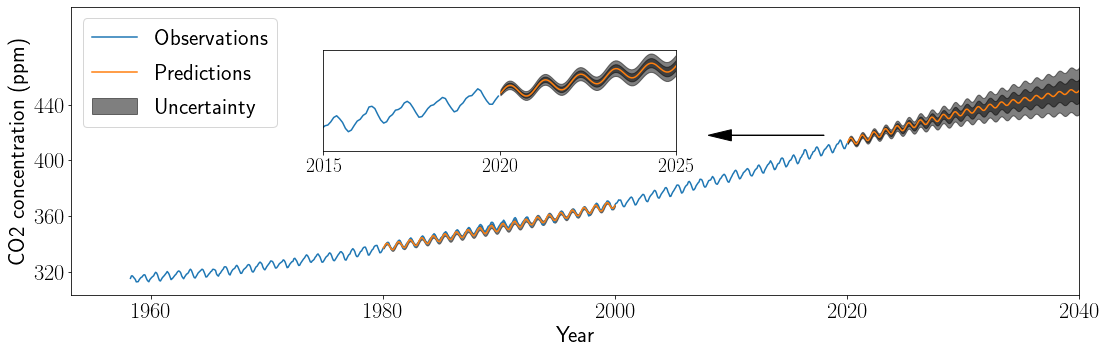
\includegraphics[width=2\columnwidth]{pics/mlc02}}
\caption{\textbf{LEG processes interpolate and extrapolate well across long timescales}.  It appears that a rank-5 LEG model is sufficient to capture the linear and periodic trends in the Mauna Loa CO$_2$ dataset.  Above we compare the true observations with interpolations made by the LEG model.  The gray areas encompass one and two predictive standard deviations, i.e. the LEG model's uncertainty in forecasting and extrapolating what out-of-sample observations would look like.}
\label{fig:realdata}
\end{center}
\vskip -0.2in
\end{figure*}


This apparent contradiction -- RQ is profoundly different (on the tails of the spectrum) from every LEG kernel, yet every RQ kernel can be matched arbitrarily well by a LEG kernel -- is resolved by considering the different timescales involved in any Gaussian Process.  LEG kernels can uniformly approximate any stationary covariance, which means that we can use them to get uniformly accurate forecasts and interpolations at any fixed timescale.  If a LEG kernel is trained on observations at a particular timescale, the kernel will attempt to match smoothness \emph{at that timescale}.  For example, these LEG kernels were trained on observations at a timescale of $.1$, so they will attempt to match the covariance at that scale and larger.


The case of the (RBF) kernel, given by $C_\mathrm{RBF}(\tau)=\exp(-\tau^2/2)$, is even more extreme.  This kernel's spectrum decays log-quadratically -- even faster than the spectrum of the RQ kernel.  For any RBF process, any RQ process, and any PEG process, one can always find a small enough scale so that the RBF process will look smoother than the RQ process and the RQ process is smoother than the PEG processes.  Modeling this smoothness is difficult for lower-rank LEG models.  For example, the best rank-2 LEG model includes a large oscillation that is not found in the ground-truth RBF kernel.  It is not until rank 4 that the LEG process is able to match the kernel well.

Finally, the Matern kernel with $\nu=1.5$ turns out to be an easy case.  This kernel is given by 
\[
C_{\mathrm{Matern}}(\tau) = (1+\sqrt{3}\tau)\exp(-\sqrt{3}\tau).
\]
Like PEG kernels, the spectrum of the Matern kernel decays slower than exponentially.  In fact, this Matern kernel lies inside the rank-2 LEG family.  Let
\[
N=3^{1/4}\left(\begin{array}{cc}
1 & -1\\
-1 & 1
\end{array}\right)\qquad R=\sqrt{3}\left(\begin{array}{cc}
0 & 1\\
-1 & 0
\end{array}\right).
\]
Then the Matern kernel is given by $\LEG(N,R,\mathbf{1}/\sqrt{2},0)$.



\begin{figure*}
\vskip 0.2in
\begin{center}
\centerline{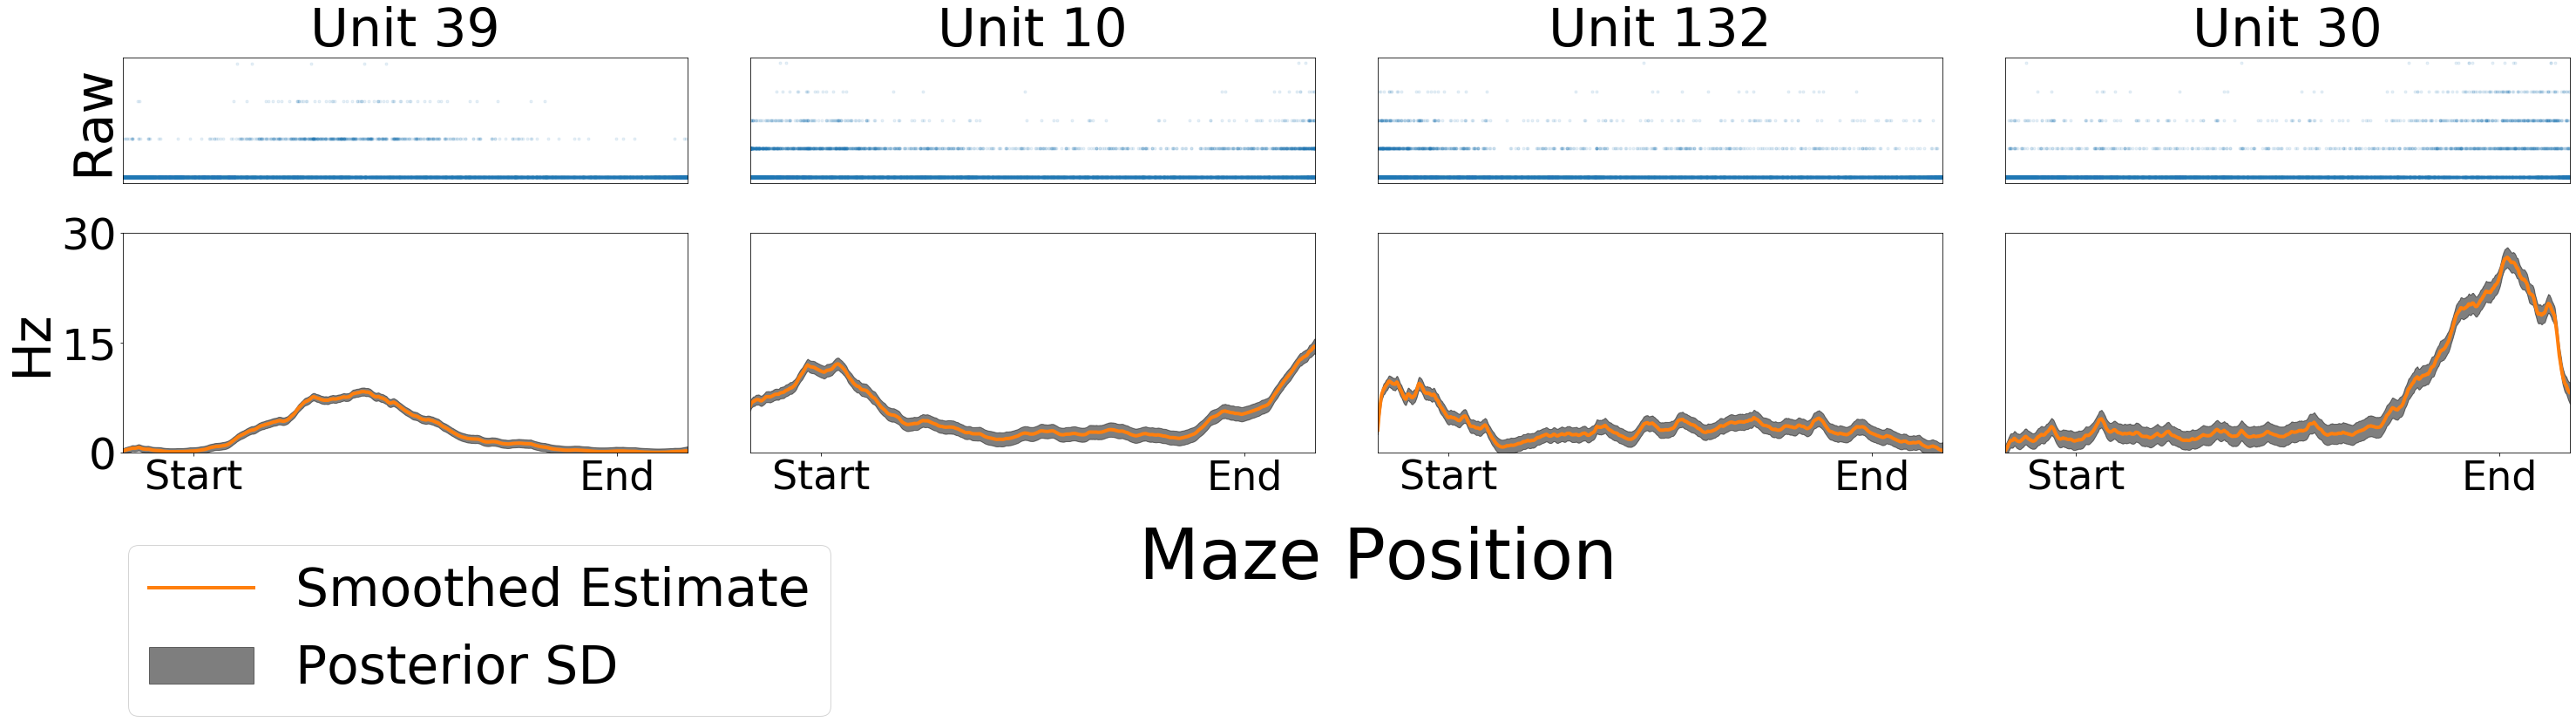
\includegraphics[width=2\columnwidth]{pics/kenny}}
\caption{\textbf{LEG processes can smooth irreguarly spaced neural data}.  Ten thousand irregularly spaced observations suggest that the firing rates of hippocampal neurons are modulated by the rat's position in a maze.  However, the modulation strength visible in the raw data is weak.  By smoothing this data with a LEG process we can see the trend more clearly. How much should we smooth?  By training a rank-5 LEG process we can determine a smoothness level automatically. The gray areas indicate the LEG model's posterior uncertainty about the estimated tuning curve.}
\label{fig:kenny}
\end{center}
\vskip -0.2in
\end{figure*}

\subsection{Mauna Loa CO$_2$}


To find out whether LEG models can offer a practical tool for extrapolation and interpolation, we turn to the Mauna Loa CO$_2$ dataset.  For the last sixty years, the monthly average atmosphere CO$_2$ concentrations at the the Mauna Loa Observatory in Hawaii have been recorded \cite{keeling2005atmospheric}.  This dataset is interesting because it features two different kinds of structures: an overall upward trend and a yearly cycle.  To test the ability of the LEG model to learn these kinds of structures from data, we trained a rank-5 LEG kernel on all the data before 1980 and all the data after 2000.  We then asked the LEG model to interpolate what happened in the middle and forecast what the concentration might look like in the next twenty years.  

The results are shown in Figure \ref{fig:realdata}.  It is encouraging that the LEG predictions interpolate adequately from 1980 to 1920.  Even though the LEG process is given no exogenous information about  ``years'' or ``seasons,'' it correctly infers the number of number of bumps between 1980 and 1920.  This example shows that the LEG model is sufficiently flexible to learn unanticipated structures in the data.  

\subsection{Hippocampal place-cells}

Smoothing is another common application of GPs.  Here we see whether LEG models can be used to smooth irregularly spaced observations from neural spiking data \cite{grosmark2016diversity}.  

In this data a rat's position in a one-dimensional maze is reported on a regular schedule, around 40 times per second.  At each time-step, each neuron may be silent or may fire (``spike'') some number of times.  For each neuron, we would like to estimate the ``tuning curve'' -- a function which takes in positions and returns the expected number of spikes as a function of the rat's position.  With no smoothness assumptions on this function, the problem is impossible; the rat is never observed at exactly the same place twice.  However, it is unclear how much smoothness should be assumed.  Gaussian Processes offer a natural way to automatically learn an appropriate level of smoothness from the data itself.  Note that the observed positions do not fall into a regularly spaced grid, so classical approaches such as the ARMA model cannot be applied.  

Here we model this tuning curve using a PEG process, $z\sim \PEGGP(N,R)$.  In this view, each data-point from the experiment constitutes a noisy observation of $z$.  When the rat is at position $t$  we model the distribution on the number of spikes observed in a small timebin as a Gaussian, with mean $B z(t)$ and variance $\Lambda \Lambda^\top$.  (It would be interesting to apply a non-Gaussian observation model here, as in, e.g., \cite{smith2003estimating,rad2010efficient,savin2016,gao2016linear}, and references therein; 
as noted in section \ref{sec:extensions}, linear-time approximate inference is feasible in this setting and is an important direction for future work.)

For each neuron we train the parameters of a separate LEG model.  We can then look at the posterior distribution on the underlying tuning curve $z$.  The posterior mean of this process for various neurons is shown in Figure \ref{fig:kenny}.  We also represent one standard-deviation of the posterior variance of $z$ with gray shading.   Fitting the LEG model and looking at the posterior under the learned model appears to yield an effective Empirical Bayes approach for this kind of data. 

\section{Conclusion}

We here make two advances in speeding up inference for Gaussian Processes on one dimension.  First, we show that the LEG model, a particularly tractable continuous-time Gaussian hidden Markov process, can be used to approximate any GP with a stationary integrable continuous kernel, critically enabling linear runtime scaling in the number of observations.  Second, we make this theoretical result practical by developing Cyclic Reduction-based algorithms to parallelize this computation, and sharing TensorFlow2-based implementations of these algorithms.  We believe these advances will open up a wide variety of new applications for GP modeling in highly data-intensive areas involving data sampled at high rates and/or over long intervals, including geophysics, astronomy, high-frequency trading, molecular biology, neuroscience, and more.

\section*{Acknowledgements}

Thanks to Jake Soloff for resolving a thorny point about matrix-valued measures.    

\bibliography{refs}
\bibliographystyle{icml2019}



\end{document}